\section{Best Pratice 1 : Rédaction d'une procédure}

Une procédure doit décrire \textbf{complètement} ce que l'on fait et de manière générique.

\subsection{Informations à inclure}
  \subsubsection{Informations administratives}
    \begin{itemize}
      \item Nom de l'entreprise
      \item Titre de la procédure
      \item Indice de révision
      \item Noms des rédacteurs
      \item Noms du responsable qualité
      \item Pagination
    \end{itemize}
  \subsubsection{Informations relatives à la procédure}
    \begin{itemize}             
      \item Responsabilités : 
        \begin{itemize}             
          \item Qui : Les acteurs et les tâches
          \item Quand : Les échéants
          \item Où : Où se situe le problème?
          \item Combien : le dimensionnement\\
        \end{itemize}
      \item Moyens (outils)
      \item Démarche (Comment?)
      \item $\rightarrow$ Résultat attendu (le Quoi)
     \end{itemize}
     
\subsection{Bonnes pratiques}

          \begin{tabular}{|p{7cm}|p{7cm}|} \hline
             Objectif d'une procédure & Bonne pratique pour y parvenir\\ \hline
             Clarifier la responsabilité et le rôle des acteurs au sein des entités, ainsi que les relations entre elles,
             dans le but d'atteindre des allégements et des simplifications administratives
             & Formuler clairement et ordonner les actions chronologiquement\\ \hline
             Raccourcir les circuits de décisions
             & Rendre la démarche répétable le plus possible\\ \hline
             Rendre efficace les meilleures pratiques
             & Assurer une bonne diffusion du document et vérifier la prise en compte de la part des différents acteurs.\\ \hline
          \end{tabular}
           \\\\
           

\par Une procédure est rarement linéaire. A un certains moment de la procédure un choix peut se faire entre plusieurs cas. Prévoir ces différents
cas permet d'optimiser le temps de traitement. Tous les cas doivent être prévu. Prenons pour exemple une procédure de réception de la monnaie.
Deux cas peuvent se présenter : soit le client donne la somme exacte qu'il doit et la procédure est finie, soit il donne plus auquel cas il 
faut gérer le rendu de la monnaie. Si c'est deux cas sont bien décrit, la procédure est rapide et efficace.           \\
\par Pour qu'une procédure soit facile à comprendre, rien de mieux qu'un schéma. Le logigramme reste la représentation la plus simple d'appréhension
permettant de visualiser un enchainement d'actions. \\

\begin{figure}[!h] %on ouvre l'environnement figure
\begin{center}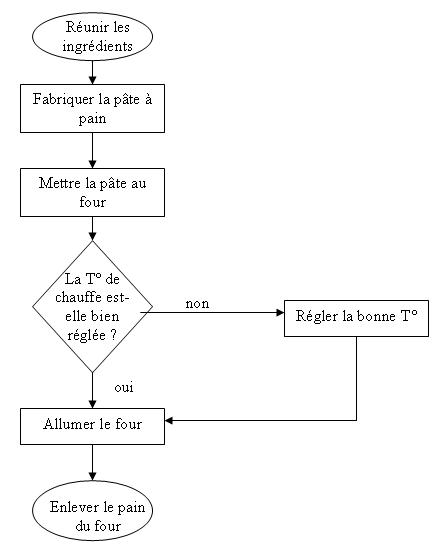
\includegraphics[height=5cm]{logigramme.jpg}\end{center}
\caption{Exemple de logigramme}
\end{figure} %on ferme l'environnement figure
\par Des procédures \textbf{claires} seront une aide appréciée et efficace (contrairement à un texte trop formel). Pour cela, l'utilisateur doit
être au coeur de la rédaction : le langage graphique et le vocabulaire utilisé doit être facilement lu par celui-ci.\\
\par Une procédure représente le \textbf{Q}ui fait \textbf{Q}uoi, \textbf{O}ù, \textbf{Q}uand, \textbf{C}omment, \textbf{C}ombien et \textbf{P}ourquoi? (QQOQCCP).
Chaque processus doit être décrit par une procédure : il s'agit là d'écrire le \textbf{"juste nécessaire"} pour sa compréhension. Ceci implique
qu'une procédure peut évoluée au cours du temps.
